\chapter{Pflichtenheft}
Bei der Erstellung dieses Pflichtenheftes wurde sich an folgendem Beispiel von Stefan Baur orientiert.\footnote{http://www.stefan-baur.de/cs.se.pflichtenheft.beispiel.html?glstyle=2010}

\section{Zielbestimmungen}
\subsection{Projektbeteiligte}
Wer soll an dem Projekt teilnehmen?
\begin{itemize}
        \item Christopher Pahl
        \item Christoph Piechula
        \item Eduard Schneider
        \item Marc Tigges
\end{itemize}
\subsection{Muss-Kriterien}
\renewcommand{\labelitemi}{•}
\begin{itemize}
	\item Verbindungsaufbau
	\item Durchführung benutzerspezifischer Client-Einstellungen
	\item Musik-Steuerung
	\item Warteschlangenverwaltung
	\item Playlistverwaltung
	\item Datenbankverwaltung
	\item Frontend für die Settings
	\item Statistikanzeige
	\item Verwaltung der Ausgabegeräte
\end{itemize}
\subsection{Wunsch-Kriterien}
\begin{itemize}
	\item Anzeige von Onlinecontent (Albencover, Lyrics etc.) unter Verwendung von libglyr\footnote{https://github.com/sahib/glyr}
\end{itemize}

\section{Produkteinsatz}
Welche Anwendungsbereiche (Zweck), Zielgruppen (Wer mit welchen Qualifikationen), Betriebsbedingungen (Betriebszeit,
Aufsicht)?\ \\ \\
Der MPD-Client ist nicht auf bestimmte Gewerbe beschränkt, ein jeder soll diesen Client
verwenden können. 
Die Software soll unter folgender Lizenz stehen:
Version 3 vom 29 Juni 2007.\ \\ \\
Definition der GPL:
\begin{center}
http://www.gnu.org/licenses/gpl.html
\end{center}
\subsection{Anwendungsbereiche}
Einzelpersonen verwenden dieses System überall da, wo mit
einem Unix-artigen Betriebssystem Musik abgespielt werden soll.
Das wären z.B. Personal Computer, Musikanlagen, Laptops und evtl.
sogar diverse Smartphones möglich.

\subsection{Zielgruppen}
Personengruppen die komfortabel von überall aus auf ihre Musik und Playlist zugreifen
wollen ohne diese jedes mal aufwändig synchronisieren zu müssen (z.B. durch Abgleich von Datenträgern). 
Aufgrund der für das System vorgesehenen Betriebsumgebung sind ebenso Kenntnisse im Umgang mit Unix nötig. 
Der Benutzer muss die Systemsprache Englisch beherrschen.


\subsection{Betriebsbedingungen}
Das System soll sich bezüglich der Betriebsbedingungen nicht sonderlich von vergleichbaren Systemen bzw.
Anwendungen unterscheiden und dementsprechend folgende Punkte erfüllen:
\begin{itemize}
        \item Betriebsdauer: Täglich, 24 Stunden
        \item Keinerlei Wartung soll nötig sein
        \item Sicherungen der Konfiguration müssen vom Benutzer vorgenommen werden
\end{itemize}

\section{Produktumgebung}
\subsection{Software}
\begin{itemize}
	\item Unixodes Betriebssystem
	\item MPD-Server 
	\item Avahi Daemon
	\item Benötigte Bibliotheken können statisch einkompiliert werden
\end{itemize}
Ein MPD-Server muss nicht unbedingt lokal installiert sein, dann muss 
allerdings über das Netzwerk (Internet) ein Server erreichbar sein.
Ohne MPD-Server soll der Client in einen definierten Zustand hochgefahren werden der das Verbinden ermöglicht.
Avahi Daemon ist optional. Er ist nicht von nöten aber durchaus praktisch wenn man sich nicht ständig den Host (bzw. die IP) 
vom Administrator geben lassen will.

\subsection{Orgware}
\begin{itemize}
	\item CMake (Buildsystem)
	\item g++ (C++ Compiler)
	\item Valgrind (Memorydebugger)
	\item git (Hosting auf Github) 
	\item Glade (GUI-Designer)
	\item doxygen  (Interne Dokumentationsgenerierung)
	\item Devhelp (Dokumentationsbrowser)
\end{itemize}

\section{Produktfunktionen}
Funktionen des MPD-Clients.\ \\
Beim ersten Start des Systems soll eine einkompilierte Standard-Konfiguration geladen werden und die Verbindungseinstellungen
zu einem MPD-Server müssen vorgenommen werden. Bei jedem weiteren Start soll die Konfiguration geladen werden,
die vom Benutzer erstellt hat,  falls keine Konfiguration gefunden wurde, oder diese korrumpiert ist,
so wird auf eine vom Client bereitgestellte Standardkonfiguration zurückgefallen. Der Benutzer soll sämtliche
Einstellungen selbstverständlich zu jeder Zeit ändern können.


Um ein Gefühl für die Funktionalität zu bekommen die der Client haben soll, wurde mit Glade ein nichtfunktionales Mockup erstellt.
Daraus sollen die finalen Features abgeleitet werden. 

\begin{figure}[h!]
    \fbox{
    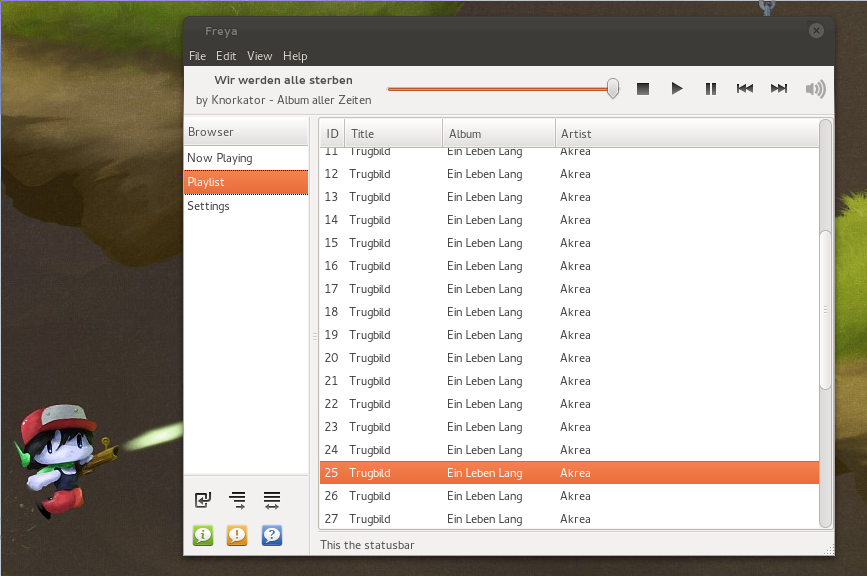
\includegraphics[width=\textwidth]{./final_mockup.png}}
    \caption{Mockup des MPD Clients}
    \label{p_mockup}
\end{figure}

Die Auflistung der Features erfolgt von links oben nach rechts unten.

\subsection{Menü}
Überall Anzeige der Keyshortcuts.
\begin{itemize}
\item File
  \begin{itemize}
  \item ,,Connect''; Insensitiv wenn bereits verbunden
  \item ,,Disconnect'', Insensitiv wenn nicht verbunden
  \item ,,Quit''
  \end{itemize} 
\item ,,Playback'' Anzeige mit Haken falls aktiviert 
  \begin{itemize}
  \item Next
  \item Previous
  \item Play
  \item Stop
  \item Consume, Single, Random, Repeat -
  \end{itemize}   
\item Misc
  \begin{itemize}
  \item ,,Increase Volume''
  \item ,,Decrease Volume''
  \end{itemize}
\item Help
  \begin{itemize}
  \item About Dialog
  \end{itemize}
\end{itemize}

%-------------------------------------------------------------

\subsection{Titelbar}
\begin{itemize}
	\item Anzeige des Musiktitels
	\begin{itemize}
		\item Benutzerhinweis wenn Client nicht verbunden ist
	\end{itemize}
	\item ,,Timeslider''
	\begin{itemize}
		\item Zeigt die aktuelle Liedposition an
		\item Durch klicken Sprung an bestimmte Musikposition möglich
		\item Bei Stop wird Slider auf 0 gesetzt, bei Pause  bleibt dieser stehen
	\end{itemize}
	
	\item Steuerbuttons
	\begin{itemize}
		\item Stopbutton - Stoppt Lied, setzt Timeslide zurück)
		\item Pausebutton - zeigt ,,play icon'' wenn pausiert und ,,stop icon'' bei Wiedergabe
		\item Pervious - vorheriges Lied
		\item Next - nächtes Lied
		\item Volumebutton - Popupslider zum regeln der Lautstärke
	\end{itemize}
	\item Untere Zeile
	\begin{itemize}
               \item Anzeige von ,,by (Artist) on (Album) ((Erscheinungsjahr))''
               \item Falls nicht connected oder nicht spielend soll ,,Not Playing angezeigt''
        \end{itemize}		
\end{itemize} 

%-------------------------------------------------------------

\subsection{Sidebar}
Die Sidebar befindet sich links und zeigt eine Liste verfügbarer Browser
\begin{itemize}
  \item Bei Klick auf einem Browser wird er ausgewählt
  \item der Inhalt wird im Pane daneben angezeigt
  \item Sollte die Browserliste überfüllt sein wird ein Scrollbalken angezeigt
\end{itemize}
Nach einem Separator findet sich ein inaktives widget das den Song anzeigt der als nächstes spielen wird.
Falls kein nächster Song wird eine entsprechende Nachricht angezeigt.
Darunter findet sich 4 eindrückbare Buttons die eindrückbar sind:
\begin{itemize}
  \item Repeat
  \item Consume
  \item Repeat
  \item Single
\end{itemize}
Falls diese Buttons beispielsweise in einem anderen Client aktiviert werden, 
so sollen die Änderungen automatisch durch die Eindrückung angezeigt werden.


%-----------------------------------------------

\subsection{Playlistmanager}
Zeigt alle vorhandenen auf dem Server gespeicherten Playlisten in einer Liste.
Dabei wird in der Liste der Playlistname und das letzte Änderungsdatum angezeigt.
Die Namenszellen sind editierbar, sodass der Playlistname einfach geändert werden kann. 
Ein Rechtsklickmenü bietet soll die folgenden Operationen bieten:
 \begin{itemize}
   \item Append: Fügt den Inhalt der Playliste der Queue am Ende hinzu
   \item Replace: Ersetzt den Inhalt der Queue mit dieser Playlist
   \item Delete: Entfernt die ausgewählten Playlisten unwiderruflich
 \end{itemize}   

%-----------------------------------------------

\subsection{Databasebrowser}
Der Databasebrowser zeigt eine Visualisierung der Datenbank die an einen Filebrowser angelehnt ist.
\footnote{Es handelt sich hierbei nicht wirklich um ein Dateisystem, nur um eine Darstellung der Musikfiles des Ordners, der in der Konfigurationsdatei des MPD-Servers also Musik-Ordner festgelegt wurde}
\begin{itemize}
   \item Anzeige von Songs und Files durch unterschiedliche Icons
   \item Anzeige des "Dateinamen" unter dem Icon
   \item Doppelklick oder Enter auf einen Ordner bewirkt ein Absteigen in diesem
   \item Doppelklick oder Enter auf ein Songfile bewirkt ein Hinzufügen dessen zur Ende der Queue
   \item 'Backspace' geht ebenso ein Verzeicniss nach oben.
   \item Am unteren Rand befindet sich eine Steuerleiste:
   \begin{itemize}
     \item homebutton: Geht zum Wurzelverzeichniss zurück
     \item Zurückbutton: Dasselbe wie backspace
     \item Das Suchfeld filtert die momentane Anzeige
     \item ganze rechts zeigt ein Label den aktuellen Pfad an
   \end{itemize}
   \item Ein Kontextmenü bietet folgende Optionen:
   \begin{itemize}
     \item Add: Fügt die ausgewählte Menge der Queue hinzu, rekursiv falls sich Verzeichnisse darunter befinden
     \item Add All: Fügt alles, ungeachtet der auswahl der queue hinzu (performatere Version von add)
     \item Replace: Wie add, löscht aber vorher die Queue
     \item Update: Weist den Server an die Datenbank zu aktualisieren, und neue/veränderte files zu aktualisieren
     \item Rescan: Weist den Server die Datenbank zu aktualisieren; untersucht alle files von neuen (teuer)
   \end{itemize}
\end{itemize}

%-----------------------------------------------

\subsection{Queue}	
\begin{itemize}
    \item Zeigt die aktuelle Warteschlange an
        \begin{itemize}
            \item Künstler, Album und Musiktitel
            \item Spalten der Queue sind frei anordenbar
        \end{itemize}
    \item Auswahl erfolgt durch linksklick (kombiniert mit shift/strg) oder durch Auswählen mit der Maus (,,Rubberbanding'')
    \item Ein Rechtsklickmenü bietet die folgenden Möglichkeiten:
        \begin{itemize}
            \item Remove: Entfernen der Songs aus der Queue
            \item Clear: Entfernen aller Songs aus der Queue
            \item Save as playlist: Die gesamte Queue wird als playlist abgespeicher, \\
                  der name der neuen playlist wird durch einen Dialog abgefragt.
        \end{itemize}
    \item Bei Änderungen des Server wird die Queue im Hintergrund geupdatet
\end{itemize}

%-----------------------------------------------

\subsection{Settingsbrowser}
Die Einstellungen sollen in ein Tabbasiertes Layout eingebettet sein. 
Werden Änderungen vorgenommen, so werden sie nicht gleich gespeichert und übernommen. 
Es sollte daher ein Speicherfunktion geben, und dazugehörig eine Undofunktion für die letzten Änderungen.
\\
Falls dem Client die Verbindung verloren soll zum Settingsbrowser gesprungen werden, sodass der Benutzer entsprechende
Änderungen machen kann. Aus diesem Grunde muss der Settingsbrowser auch ohne Verbindung voll funktionsfähig sein.
Alle Settingstabs ändern die Werte nicht sofort:
\begin{itemize} 
   \item Sie werden erst persistent übernommen wenn der user die Konfiguration abspeichert
   \item Der Rückgängig button setzt die Präsentation auf die letzen persistent gesetzten Werte
   \item "Zurücksetzen" lädt überall die Defaultconfig
\end{itemize}
Innerhalb der Tabs sollen folgende Funktionen bereit gestellt werden:
\begin{itemize}
	\item Der Benutzer kann Netzwerk-Einstellungen vornehmen
	\begin{itemize}
		\item Server IP / Port
		\item Avahi-Browser (Serverliste)
		\item Autoconnect
	\end{itemize}
	\item Der Benutzer kann Playback-Einstellungen vornehmen	
	\begin{itemize}
		\item Crossfade in Sekunden (Weicher Übergang zwischen jetzigem und nächstem Lied)
		\item Musik beim verlassen stoppen
	\end{itemize}
	\item Der Benutzer kann Allgemein-Einstellungen vornehmen
	\begin{itemize}
		\item Notifications(libnotify) nutzen, falls ja auch wie lange diese angezeigt werden
		\item Tray-Icon anzeigen
	\end{itemize}
	\item Der Benutzer soll eine Audioausgabeliste haben:
	\begin{itemize}
		\item Innerhalb der Liste soll es Checkboxes geben um den output entweder an oder auszuschalten
		\item Dies soll nicht verfügbar sein wenn die Verbindung verloren geht
	\end{itemize}
\end{itemize}

\subsubsection{Fußleiste}
Falls verbunden zeigt sie:
\begin{itemize}
	\item Samplingrate in Khz
	\item Audiobitrate in Kbit
	\item Outputart (serverbedingt kann nur Stereo oder Mono angezeit werden, 5.1 Audiofiles werden auch als Stereo dargestellt)
	\item Zeit aktuell von insgesamt
	\item Anzahl an Songs in der Datenbank
	\item Komplette Abspielzeit der Datenbank
	\item Lautstärke 0-100\%
\end{itemize}
\subsubsection{Sonstiges}
\begin{itemize}
	\item D\_0060 Nächster Song (Seitenleiste)
\end{itemize}

\section{Produktdaten}

\subsection{Starten und Beenden}
\begin{itemize}
	\item Der Benutzer kann das System zu jedem Zeitpunkt starten.
	\item Der Benutzer kann das System zu jedem Zeitpunkt beenden.
	\item Beim ersten Start wird ein Standart-System-Zustand geladen.
	\item Beim Beenden wird der aktuelle System-Zustand gespeichert.
	\item Bei jedem weiteren Start wird der letzte System-Zustand geladen.
\end{itemize}
\subsection{Abspielen von Musik (Buttons)}
Der Benutzer kann
\begin{itemize}
	\item Musik abspielen (Play)
	\item Musik stoppen (Stop)
	\item Musik pausieren (Pause)
	\item Musik vor und zurück schalten (Skip)
	\item Musik vor und zurück spuhlen (Seek)
	\item Musik zufällig abspielen (Random)
	\item Musik wiederholen (Repeat)
	\item Musik im Consume-Mode abspielen
	\item Musik im Single-Mode abspielen
\end{itemize}
\subsection{Abspielen von Musik (Shortcuts)}
Folgende Shortcut sollen in der finalen Version verfügbar sein:
\begin{itemize}
	\item Play 	(ctrl + G)
        \item Stop 	(ctrl + S)
        \item Previous 	(ctrl + P)
        \item Next	(ctrl + N)
	\item Random	(ctrl + Z)
	\item Single	(ctrl + Y)
	\item Repeate	(ctrl + R)
	\item Consume	(ctrl + T)
        \item Verbinden	(ctrl + C)
	\item Trennen	(ctrl + D)
	\item Beenden	(ctrl + Q)
\end{itemize}


\subsection{Administrator-Funktionen}
Durch das Unix-artige System wird der Administrator-Zugriff geregelt. Sobald sich der Benutzer im Unix System
als Administrator befindet, kann er auch den MPD-Client administrieren. Ein zusätzlicher Administrator-Modus wurde also
nicht implementiert.

\subsection{Suchen in der Queue}
Eine einfache Textsuche zum finden von Titeln, Alben oder Interpreten innerhalb der 
Abspiellisten wurde implementiert. Dabei springt die Markierung des Textes beim 
eingeben von Zeichen in die Suche zu der ersten übereinstimmenden Stelle in der 
Plaxlist des Clients. Erst beim bestätigen der Eingabe im Suchfeld wird die Auswahl 
gefiltert.
\begin{itemize}
	\item Der Benutzer kann seine Queue durchsuchen
	\item Der Benutzer kann sein Dateisystem durchsuchen
\end{itemize}
\subsection{Statistik}
\begin{itemize}
	\item F\_0070 Der Benutzer kann eine gesamt Statistik einsehen
	\begin{itemize}
		\item Anzahl der Interpreten
		\item Anzahl der Alben
		\item Anzahl der Lieder
		\item Musiklänge der Datenbank
		\item Abspielzeit	
		\item Zeit Online bzw. mit MPD verbunden
		\item Letztes Datenbank-Update
	\end{itemize}
\end{itemize}

\subsection{Persönliches Profil}
Da die Software auf Unix-artige Systeme beschränkt ist, wurde keine Profil-Verwaltung implementiert. Die
verschiedenen Profile werden durch die verschiedenen Profile des gesamten Betriebssystems definiert und differenziert.
Für spätere Versionen könnte ergänzend auch ein Serveraddressbuch implementiert werden.
\subsection{Mehrfachstart des Clients}
Gegen mehrfaches Starten ist der Client nicht abgesichert. Die einzige Schnittmengen die mehrere Instanzen des Clients sich teilen 
liegt in der persistenten Datenspeicherung des Logs. Werden die Clients zeitversetzt gestartet sollte hier allerdings kaum etwas passieren. 
\subsection{Persönliche Datenbank}
Eine persönliche Datenbank ist lokal nicht vorhanden. Die Datenbank des Benutzers befindet sich auf dem MPD-Server.
Einzig und alleine modulare Erweiterungen des MPD-Clients können lokale Datenbank-Implementierungen erfordern.
\subsection{Persönliche Einstellungen}
Client Einstellungen werden lokal gespeichert, außerdem ist stets eine Defaultconfig vorhanden, falls die des Dateisystems defekt ist.
Die Konfigurationsdatei wird nach dem XDG-Standard in ~/.config/freya/config.xml gespeichert. Den selben Speicherplatz wählt auch die Logdatei 
(~/.config/freya/log.txt). Sollten nur einzelne Werte in der Konfigurationsdatei nicht vorhanden sein so wird nachgeschaut ob die Defaultconfig
diese Werte bereitstellt und es wird versucht sie von dort zu laden. So ist für valide Wert stets abgesichert dass mindestens ein Wert vorliegt.
\section{Qualitätsanforderungen}
Die Software soll natürlich von hoher Qualität sein. Hierfür sollen folgende
Anforderungen erfüllt werden:
\subsection{Korrektheit}
Die Software muss möglichst fehlerfrei und korrekt sein. Es wurden Testszenarien und Testfälle erstellt,
um Fehler zu finden und auszubessern. Aber auch wenn nach Veröffentlichung der Software ein 
Fehler gefunden werden sollte, wird dieser sofort ausgebessert. Bei schwerwiegenden Fehlern
werden die Nutzer direkt auf den Fehler aufmerksam gemacht.
\subsection{Wartbarkeit}
Der Wartungsaufwand der Software ist gering bis gar nicht vorhanden. Ändert sich die Umgebungssoftware
(z.B. der MPD-Server) dann sind die Änderungen so geringfügig bzw. trivial, dass sie den MPD-Client 
nicht beeinflussen werden. Fehler der Software (sollten Fehler auftreten) wären leicht analysier- bzw.
prüfbar und natürlich auch leicht zu beheben. Zur Wartbarkeit gehört ebenso die Modularität, d. h.
die Software ist technisch so realisiert, dass sie leicht erweitert werden kann, Stichwort Model View
Controller (MVC). An kritischen Stellen versuchen Fehlerbehandlungroutinen alle Fehler möglichst vollständig abzufangen. 
Alle diese Routinen schreiben Meldungen in eine Log-Datei.
\subsection{Zuverlässigkeit}
Das System funktioniert und reagiert tolerant auf fehlerhafte Eingaben bzw. fehlerhafte Benutzung.
Das Programm funktioniert sieben Tage die Woche und 24h am Tag und muss nicht abgeschaltet werden.

\subsection{Effizienz}
Der MPD-Client funktioniert möglichst effizient, d.h. das Programm ist schnell geladen und Eingaben des Benutzers
werden praktisch sofort ausgeführt. Es gibt so gut wie keine Wartezeiten, jedenfalls sind diese 
so genannten Reaktionszeiten für den Benutzer nicht merkbar. Selbst bei sehr großen Musik-Datenbanken
und Playlists benötigt das Programm kaum Rechenzeit und sonstige Hardwareressourcen.

\subsection{Benutzbarkeit}
Die Software ist leicht verständlich und intuitiv bedienbar. Nötige Kenntnisse zur Nutzung des 
MPD-Clients sind leicht zu erlernen. Hier wird allerdings davon ausgegangen dass der MPD Server bereits
fertig eingerichtet ist. Sollte dies nicht der Falls sein, so sind Fähigkeiten in der Kommandozeile 
durchaus hilfreich.

\subsection{Design}
Das Design soll ansprechend und modern sein, allerdings wenn es Konflikte zwischen technischer Umsetzung 
und Design oder Effizienz und Design geben sollte, ist stets im Interesse der technischen Umsetzung bzw. 
der Effizienz zu entscheiden.
<<<<<<< HEAD:doc/architecture/Doku/Pflichtenheft.tex

=======
\section{Globale Testszenarien und Testfälle}
\subsection{Cxxtest}
\begin{quote}
CxxTest is a JUnit/CppUnit/xUnit-like framework for C/C++.\ \\ \\
It is focussed on being a lightweight framework that is well suited for 
integration into embedded systems development projects.\ \\ \\
CxxTest's advantages over existing alternatives are that it:\ \\ \\
\begin{itemize}
	\item Doesn't require RTTI
    	\item Doesn't require member template functions
    	\item Doesn't require exception handling
	\item Doesn't require any external libraries (including memory management, file/console I/O, graphics libraries)
	\item Is distributed entirely as a set of header files (and a python script).
	\item Doesn't require the user to manually register tests and test suites 
\end{itemize}
This makes it extremely portable and usable.\ \\ \\
Currently CxxTest is about to get a major update. The stable version 
(3.10.1) is available in the documents and files section.\ \\ \\
For more information you may visit our wiki. If you are interested in 
helping this project you can start by browsing the code and looking at the 
currently open issues. 
\end{quote} \footnote{http://cxxtest.tigris.org/}
\subsubsection{Testfälle}
\subsection{Testprotokoll}
Um Fehler aufzuspühren, die die grafische Oberfläche betreffen, wurde ein Testprotokoll erstellt in dem zunächst
alle möglichen Funktionen der grafischen Oberfläche aufgelistet werden. Außerdem müssen diese Funktionen mit 
anderen Funktionen kombiniert und mehrfach ausgeführt werden. Zu jedem dieser Fälle ist ein zu erwartendes Ergebnis
festzulegen und anschließend zu überprüfen ob das erwartete Ergebnis eingetroffen ist. Das eingetroffene Ergebnis
ist ebenfalls zu protokollieren. Es wurden jeweils die Buttons, sowie die Shortcuts geprüft.
\subsubsection{Abspielfunktionen}
\textbf{Einfache Ausführung:}\ \\ \\
\begin{tabular}[c]{|l|p{6cm}|c|}
\hline
\textbf{Testfall} & \textbf{Erwartetes Ergebnis} & \textbf{Ergebnis eingetroffen?}\\
\hline
Play & Musik spielt ab.\newline Play wird zu Pause. & Ja\\
\hline
Pause & Musik pausiert.\newline Pause wird zu Play. & Ja\\
\hline
Next & Nächstes Lied abspielen & Ja\\
\hline
Previous & Vorheriges Lied abspielen & Ja\\
\hline
Stop & Beende abspielen\newline Pause wird zu Play. & Ja\\
\hline
Skipping & An Liedposition springen & Ja\\
\hline
Random & Musik der Queue zufällig abspielen & Ja\\
\hline 
Repeat & Ein Lied wiederholen & Ja\\
\hline
Repeat all & Queue wiederholen & Ja\\
\hline
Consume Mode & Ein abgespieltes Lied entfernen & Ja\\
\hline
Single Mode & Ein Lied abspielen, dann Stoppen & Ja\\
\hline
\end{tabular}
\newpage
\textbf{Kombinierte Ausführung:}\ \\ \\
\begin{tabular}[c]{|p{6cm}|p{6cm}|c|}
\hline
\textbf{Testfall} & \textbf{Erwartetes Ergebnis} & \textbf{Ergebnis eingetroffen?}\\
\hline
Play, Stop, Play(1) & Musik spielt ab.\newline Musik stoppt.\newline Musik spielt ab. & Ja\\
\hline
Play, Pause, Play(2) & Musik spiel ab.\newline Musik pausiert.\newline Musik spiel ab. & Ja\\
\hline
Next, Next(3) & Skip weiter.\newline Skip weiter. & Ja\\
\hline
Previous, Previous(4) & Skip zurück.\newline Skip zurück & Ja\\
\hline
Next, Previous(5) & Skip weiter.\newline Skip zurück & Ja\\
\hline
Previous, Next(6) & Skip zurück.\newline Skip weiter & Ja\\
\hline
Random, Repeat all & Musik der Queue zufällig abspielen\newline Queue wiederholen & Ja\\
\hline
Random, Consume Mode & Musik der queue zufällig abspielen\newline Ein abgespieltes Lied entfernen & Ja\\
\hline
Random, Single Mode & Musik der Queue zufällig abspielen\newline Ein Lied abspielen, dann stoppen & Ja\\
\hline
Consume Mode, Single Mode & Ein abgespieltes Lied entfernen\newline Ein Lied abspielen, dann Stoppen & Ja\\
\hline
Consume Mode, Repeat all & Kann nur einmal durchlaufen & Ja\\
\hline
Random, 1 & Musik der Queue zufällig abspielen\newline 1 & Ja\\
\hline
Random, 2 & Musik der Queue zufällig abspielen\newline 2 & Ja\\
\hline
Random, 3 & Musik der Queue zufällig abspielen\newline 3 & Ja\\
\hline
Random, 4 & Musik der Queue zufällig abspielen\newline 4 & Ja\\
\hline
Random, 5 & Musik der Queue zufällig abspielen\newline 5 & Ja\\
\hline
Random, 6 & Musik der Queue zufällig abspielen\newline 6 & Ja\\
\hline
Repeat all, 1 & Queue wiederholen\newline 1 & Ja\\
\hline
Repeat all, 2 & Queue wiederholen\newline 2 & Ja\\
\hline
Repeat all, 3 & Queue wiederholen\newline 3 & Ja\\
\hline
Repeat all, 4 & Queue wiederholen\newline 4 & Ja\\
\hline
\end{tabular}
\begin{tabular}[c]{|p{6cm}|p{6cm}|c|}
\hline
\textbf{Testfall} & \textbf{Erwartetes Ergebnis} & \textbf{Ergebnis eingetroffen?}\\
\hline
Repeat all, 5 & Queue wiederholen\newline 5 & Ja\\
\hline
Repeat all, 6 & Queue wiederholen\newline 6 & Ja\\
\hline
Consume Mode, 1 & Ein abgespieltes Lied entfernen\newline 1 & Ja\\
\hline
Consume Mode, 2 & Ein abgespieltes Lied entfernen\newline 2 & Ja\\
\hline
Consume Mode, 3 & Ein abgespieltes Lied entfernen\newline 3 & Ja\\
\hline
Consume Mode, 4 & Ein abgespieltes Lied entfernen\newline 4 & Ja\\
\hline
Consume Mode, 5 & Ein abgespieltes Lied entfernen\newline 5 & Ja\\
\hline
Consume Mode, 6 & Ein abgespieltes Lied entfernen\newline 6 & Ja\\
\hline
Single Mode, 1 & Ein Lied abspielen, dann Stoppen\newline 1 & Ja\\
\hline
Single Mode, 2 & Ein Lied abspielen, dann Stoppen\newline 2 & Ja\\
\hline
Single Mode, 3 & Ein Lied abspielen, dann Stoppen\newline 3 & Ja\\
\hline
Single Mode, 4 & Ein Lied abspielen, dann Stoppen\newline 4 & Ja\\
\hline
Single Mode, 5 & Ein Lied abspielen, dann Stoppen\newline 5 & Ja\\
\hline
Single Mode, 6 & Ein Lied abspielen, dann Stoppen\newline 6 & Ja\\
\hline
\end{tabular}
\newpage
Im folgenden wird auf das Protokoll der kombinierten Ausführung referenziert.\ \\ \\
\textbf{Mehrfache Ausführung:}\ \\ \\
\begin{tabular}[c]{|p{6cm}|p{6cm}|c|}
\hline
\textbf{Testfall} & \textbf{Erwartetes Ergebnis} & \textbf{Ergebnis eingetroffen?}\\
\hline
Fall 1 x 10 & Fall 1 x 10 & Ja\\
\hline
Fall 2 x 10 & Fall 2 x 10 & Ja\\
\hline
Fall 3 x 10 & Fall 3 x 10 & Ja\\
\hline
Fall 4 x 10 & Fall 4 x 10 & Ja\\
\hline
Fall 5 x 10 & Fall 5 x 10 & Ja\\
\hline
Fall 6 x 10 & Fall 6 x 10 & Ja\\
\hline
Fall 12 x 10 & Fall 12 x 10 & Ja\\
\hline
Fall 13 x 10 & Fall 13 x 10 & Ja\\
\hline
Fall 14 x 10 & Fall 14 x 10 & Ja\\
\hline
Fall 15 x 10 & Fall 15 x 10 & Ja\\
\hline
Fall 16 x 10 & Fall 16 x 10 & Ja\\
\hline
Fall 17 x 10 & Fall 17 x 10 & Ja\\
\hline
Fall 18 x 10 & Fall 18 x 10 & Ja\\
\hline
Fall 19 x 10 & Fall 19 x 10 & Ja\\
\hline
Fall 20 x 10 & Fall 20 x 10 & Ja\\
\hline
Fall 21 x 10 & Fall 21 x 10 & Ja\\
\hline
Fall 22 x 10 & Fall 22 x 10 & Ja\\
\hline
Fall 23 x 10 & Fall 23 x 10 & Ja\\
\hline
Fall 24 x 10 & Fall 24 x 10 & Ja\\
\hline
Fall 25 x 10 & Fall 25 x 10 & Ja\\
\hline
Fall 26 x 10 & Fall 26 x 10 & Ja\\
\hline
Fall 27 x 10 & Fall 27 x 10 & Ja\\
\hline
Fall 28 x 10 & Fall 28 x 10 & Ja\\
\hline 
Fall 29 x 10 & Fall 29 x 10 & Ja\\
\hline
Fall 30 x 10 & Fall 30 x 10 & Ja\\
\hline
Fall 31 x 10 & Fall 31 x 10 & Ja\\
\hline
Fall 32 x 10 & Fall 32 x 10 & Ja\\
\hline
Fall 33 x 10 & Fall 33 x 10 & Ja\\
\hline
Fall 34 x 10 & Fall 34 x 10 & Ja\\
\hline
Fall 35 x 10 & Fall 35 x 10 & Ja\\
\hline
\end{tabular}
\subsubsection{Queue-Funktionen}
\textbf{Einfache Ausführung}\ \\ \\
\begin{tabular}[c]{|p{6cm}|p{6cm}|c|}
\hline
\textbf{Testfall} & \textbf{Erwartetes Ergebnis} & \textbf{Ergebnis eingetroffen?}\\
\hline
Remove & Ein Lied aus Queue entfernen & Ja\\
\hline
Clear & Alle Lieder aus Queue entfernen & Ja\\
\hline
Save as Playlist & Queue als Playlist speichern & Ja\\
\hline
Suchen & Nach eingegebenem Wort suchen & Ja\\
\hline
\end{tabular}
\newpage
\textbf{Kombinierte Ausführung}\ \\ \\
Kombinierte Ausführung der Funktionen der Queue machen nicht wirklich viel Sinn da z.B.
die Funktion Clear die Queue löscht. Auch Save as Playlist wird wohl kaum öfter als einmal
pro Queue angewandt. Die einzige Kombination die Sinn macht getestet zu werden ist die 
folgende:\ \\ \\
\begin{tabular}[c]{|p{6cm}|p{6cm}|c|}
\hline
\textbf{Testfall} & \textbf{Erwartetes Ergebnis} & \textbf{Ergebnis eingetroffen?}\\
\hline
Suchen, Remove & Nach eingegebenem Wort suchen\newline Ein Lied aus der Queue entfernen & Ja\\
\hline
\end{tabular}
\ \\ \\
\textbf{Mehrfache Ausführung}\ \\ \\
Die mehrfache Ausführung ist ähnlich unsinnig wie die der kombinierten Ausführung.
Mehrmals hintereinander die Queue löschen ist nicht möglich, genauso wie man wohl kaum 
mehrmals die gleiche Playlist erstellt. So bleibt wieder nur ein Testfall zu prüfen:\ \\ \\
\begin{tabular}[c]{|p{6cm}|p{6cm}|c|}
\hline
\textbf{Testfall} & \textbf{Erwartetes Ergebnis} & \textbf{Ergebnis eingetroffen?}\\
\hline
Suchen, Remove x 10 & Nach eingegebenem Wort suchen\newline Ein Lied aus der Queue entfernen x 10& Ja\\
\hline
\end{tabular}
\subsubsection{Playlist-Funktionen}
\textbf{Einfache Ausführung}\ \\ \\
\begin{tabular}[c]{|p{6cm}|p{6cm}|c|}
\hline
\textbf{Testfall} & \textbf{Erwartetes Ergebnis} & \textbf{Ergebnis eingetroffen?}\\
\hline
Hinzufügen & Playlist zur Queue hinzufügen & Ja\\
\hline
Ersetzen & Queue durch Playlist ersetzen & Ja\\
\hline
Playlist entfernen & Playlist löschen & Ja\\
\hline
\end{tabular}
\ \\ \\
\textbf{Kombinierte Ausführung}\ \\ \\
\begin{tabular}[c]{|p{6cm}|p{6cm}|c|}
\hline
\textbf{Testfall} & \textbf{Erwartetes Ergebnis} & \textbf{Ergebnis eingetroffen?}\\
\hline
Hinzufügen, Hinzufügen & Playlist zur Queue hinzufügen\newline Playlist zur Queue hinzufügen & Ja\\
\hline
Ersetzen, Ersetzen & Queue durch Playlist ersetzen\newline Queue durch Playlist ersetzen & Ja\\
\hline
Entfernen, Entfernen & Playlist entfernen\newline Playlist entfernen & Ja\\
\hline
Hinzufügen, Entfernen & Playlist zur Queuehinzufügen\newline Playlist löschen & Ja\\
\hline
Ersetzen, Entfernen & Queue durch Playlist ersetzen\newline Playlist entfernen & Ja\\
\hline
\end{tabular}
\newpage
Im folgenden wird auf das Protokoll der kombinierten Ausführung referenziert.\ \\ \\
\textbf{Mehrfache Ausführung:}\ \\ \\
\begin{tabular}[c]{|p{6cm}|p{6cm}|c|}
\hline
\textbf{Testfall} & \textbf{Erwartetes Ergebnis} & \textbf{Ergebnis eingetroffen?}\\
\hline
Fall 1 x 10 & Fall 1 x 10 & Ja\\
\hline
Fall 2 x 10 & Fall 2 x 10 & Ja\\
\hline
Fall 3 x 10 & Fall 3 x 10 & Ja\\
\hline
Fall 4 x 10 & Fall 4 x 10 & Ja\\
\hline
Fall 5 x 10 & Fall 5 x 10 & Ja\\
\hline
\end{tabular}
\subsubsection{Dateibrowser-Funktionen}
\textbf{Einfache Ausführung}\ \\ \\
\begin{tabular}[c]{|p{6cm}|p{6cm}|c|}
\hline
\textbf{Testfall} & \textbf{Erwartetes Ergebnis} & \textbf{Ergebnis eingetroffen?}\\
\hline
Hinzufügen & Zur Queue hinzufügen & Ja\\
\hline
Alle Hinzufügen & Alle zur Queue hinzufügen & Ja\\
\hline
Ersetzen & Queue durch Auswahl ersetzen & Ja\\
\hline
Aktualisieren & Dateibrowser aktualisieren & Ja\\
\hline
Neu einlesen & Dateibrowser neu einlesen & Ja\\
\hline
Suchen & Nach eingegebenem Wort suchen & Ja\\
\hline
\end{tabular}
\ \\ \\
\textbf{Kombinierte Ausführung}\ \\ \\
\begin{tabular}[c]{|p{6cm}|p{6cm}|c|}
\hline
\textbf{Testfall} & \textbf{Erwartetes Ergebnis} & \textbf{Ergebnis eingetroffen?}\\
\hline
Hinzufügen\newline Hinzufügen & Zur Queue hinzufügen\newline Zur Queue hinzufügen & Ja\\
\hline
Alle Hinzufügen\newline Alle hinzufügen &  Alle zur Queue hinzufügen\newline Alle zur Queue hinzufügen & Ja\\
\hline
Ersetzen\newline Ersetzen & Queue durch Auswahl ersetzen\newline Queue durch Auswahl ersetzen & Ja\\
\hline
Aktualisieren\newline Aktualisieren & Dateibrowser aktualisieren\newline Dateibrowser aktualisieren & Ja\\
\hline
Neu einlesen\newline Neu einlesen & Dateibrowser neu einlesen\newline Dateibrowser neu einlesen & Ja\\
\hline
Suchen\newline Suchen & Nach eingegebenem Wort suchen\newline Nach eingegebenem Wort suchen & Ja\\
\hline
Hinzufügen\newline Alle Hinzufügen & Zur Queue hinzufügen\newline Alle zur Queue hinzufügen & Ja\\
\hline
Hinzufügen\newline Ersetzen & Zur Queue hinzufügen\newline Queue durch Auswahl ersetzen & Ja\\
\hline
Hinzufügen\newline Aktualisieren & Zur Queue hinzufügen\newline Dateibrowser aktualisieren & Ja\\
\hline
Hinzufügen\newline Neu einlesen & Zur Queue hinzufügen\newline Dateibrowser neu einlesen & Ja\\
\hline
\end{tabular}
\begin{tabular}[c]{|p{6cm}|p{6cm}|c|}
\hline
\textbf{Testfall} & \textbf{Erwartetes Ergebnis} & \textbf{Ergebnis eingetroffen?}\\
\hline
Hinzufügen\newline Suchen & Zur Queue hinzufügen\newline Nach eingegebenem Wort suchen & Ja\\
\hline
Alle Hinzufügen\newline Ersetzen & Alle zur Queue hinzufügen\newline Queue durch Auswahl ersetzen & Ja\\
\hline
Alle Hinzufügen\newline Aktualisieren & Alle zur Queue hinzufügen\newline Dateibrowser aktualisieren & Ja\\
\hline
Alle Hinzufügen\newline Neu einlesen & Alle zur Queue hinzufügen\newline Dateibrowser neu einlesen & Ja\\
\hline
Alle Hinzufügen\newline Suchen & Alle zur Queue hinzufügen\newline Nach eingegebenem Wort suchen & Ja\\
\hline
Ersetzen\newline Aktualisieren & Queue durch Auswahl ersetzen\newline Dateibrowser aktualisieren & Ja\\
\hline
Ersetzen\newline Neu einlesen & Queue durach Auswahl ersetzen\newline Dateibrowser neu einlesen & Ja\\
\hline
Ersetzen\newline Suchen & Queue durch Auswahl ersetzen\newline Nach eingegebenem Wort suchen & Ja\\
\hline
Aktualisieren\newline Neu einlesen & Dateibrowser aktualisieren\newline Dateibrowser neu einlesen & Ja\\
\hline
Aktualisieren\newline Suchen & Dateibrowser aktualisieren\newline Nach eingegebenem Wort suchen & Ja\\
\hline
Neu einlesen\newline Suchen & Dateibrowser neu einlesen\newline Nach eingegebenem Wort suchen & Ja\\
\hline
\end{tabular}
\ \\ \\
Im folgenden wird auf das Protokoll der kombinierten Ausführung referenziert.\ \\ \\
\textbf{Mehrfache Ausführung}\ \\ \\
\begin{tabular}[c]{|p{6cm}|p{6cm}|c|}
\hline
\textbf{Testfall} & \textbf{Erwartetes Ergebnis} & \textbf{Ergebnis eingetroffen?}\\
\hline
Fall 1 x 10 & Fall 1 x 10 & Ja\\
\hline
Fall 2 x 10 & Fall 2 x 10 & Ja\\
\hline
Fall 3 x 10 & Fall 3 x 10 & Ja\\
\hline
Fall 4 x 10 & Fall 4 x 10 & Ja\\
\hline
Fall 5 x 10 & Fall 5 x 10 & Ja\\
\hline
Fall 6 x 10 & Fall 6 x 10 & Ja\\
\hline
Fall 7 x 10 & Fall 7 x 10 & Ja\\
\hline
Fall 8 x 10 & Fall 8 x 10 & Ja\\
\hline
Fall 9 x 10 & Fall 9 x 10 & Ja\\
\hline
Fall 10 x 10 & Fall 10 x 10 & Ja\\
\hline
\end{tabular}
\begin{tabular}[c]{|p{6cm}|p{6cm}|c|}
\hline
\textbf{Testfall} & \textbf{Erwartetes Ergebnis} & \textbf{Ergebnis eingetroffen?}\\
\hline
Fall 11 x 10 & Fall 11 x 10 & Ja\\
\hline
Fall 12 x 10 & Fall 12 x 10 & Ja\\
\hline
Fall 13 x 10 & Fall 13 x 10 & Ja\\
\hline
Fall 14 x 10 & Fall 14 x 10 & Ja\\
\hline
Fall 15 x 10 & Fall 15 x 10 & Ja\\
\hline
Fall 16 x 10 & Fall 16 x 10 & Ja\\
\hline
Fall 17 x 10 & Fall 17 x 10 & Ja\\
\hline
Fall 18 x 10 & Fall 18 x 10 & Ja\\
\hline
Fall 19 x 10 & Fall 19 x 10 & Ja\\
\hline
Fall 20 x 10 & Fall 20 x 10 & Ja\\
\hline
Fall 21 x 10 & Fall 21 x 10 & Ja\\
\hline
\end{tabular}
\subsubsection{Statistik}
Für die Statistik kann kein Testprotokoll angewandt werden.
\subsubsection{Einstellungen}
\textbf{Einfache Ausführung}\ \\ \\
\begin{tabular}[c]{|p{6cm}|p{6cm}|c|}
\hline
\textbf{Testfall} & \textbf{Erwartetes Ergebnis} & \textbf{Ergebnis eingetroffen?}\\
\hline
Zeige Liste & Zeige Avahi Liste & Ja\\
\hline
\end{tabular}
\ \\ \\
\textbf{Kombinierte Ausführung}\ \\ \\
Es existieren keine Buttons oder Shortcuts die kombiniert werden könnten.\ \\ \\
\textbf{Mehrfache Ausführung}\ \\ \\
\begin{tabular}[c]{|p{6cm}|p{6cm}|c|}
\hline
\textbf{Testfall} & \textbf{Erwartetes Ergebnis} & \textbf{Ergebnis eingetroffen?}\\
\hline
Fall 1 x 10 & Fall 1 x 10 & Ja\\
\hline
\end{tabular}
\subsubsection{Lautstärke}
\textbf{Einfache Ausführung}\ \\ \\
\begin{tabular}[c]{|p{6cm}|p{6cm}|c|}
\hline
Lautstärke erhöhen & Lautstärke erhöhen & Ja\\
\hline
Lautstärke verringern & Lautstärke verringern & Ja\\
\hline
\textbf{Testfall} & \textbf{Erwartetes Ergebnis} & \textbf{Ergebnis eingetroffen?}\\
\hline
\end{tabular}
\ \\ \\
\textbf{Kombinierte Ausführung}\ \\ \\
\begin{tabular}[c]{|p{6cm}|p{6cm}|c|}
\hline
\textbf{Testfall} & \textbf{Erwartetes Ergebnis} & \textbf{Ergebnis eingetroffen?}\\
\hline
Lautstärke erhöhen\newline Lautstärke verringern & Lautstärke erhöhen\newline Lautstärke verringern & Ja\\
\hline
\end{tabular}
\ \\ \\
Im folgenden wird auf das Protokoll der kombinierten Ausführung referenziert.\ \\ \\
\textbf{Mehrfache Ausführung}\ \\ \\
\begin{tabular}[c]{|p{6cm}|p{6cm}|c|}
\hline
\textbf{Testfall} & \textbf{Erwartetes Ergebnis} & \textbf{Ergebnis eingetroffen?}\\
\hline
Fall 1 x 10 & Fall 1 x 10 & Ja\\
\hline
\end{tabular}
\subsubsection{Sonstiges}
\textbf{Einfache Ausführung}\ \\ \\
\begin{tabular}[c]{|p{6cm}|p{6cm}|c|}
\hline
\textbf{Testfall} & \textbf{Erwartetes Ergebnis} & \textbf{Ergebnis eingetroffen?}\\
\hline
Verbinden & Verbindung zum MPD-Server & Ja\\
\hline
Trennen & Verbindung zum Server trennen & Ja\\
\hline
Beenden & MPD-Client beenden & Ja\\
\hline
\end{tabular}
\ \\ \\
\textbf{Kombinierte Ausführung}\ \\ \\
\begin{tabular}[c]{|p{6cm}|p{6cm}|c|}
\hline
\textbf{Testfall} & \textbf{Erwartetes Ergebnis} & \textbf{Ergebnis eingetroffen?}\\
\hline
Verbinden\newline Verbinden & Verbindung zum MPD-Server\newline Verbindung zum MPD-Server & Ja\\
\hline
Verbinden\newline Trennen & Verbindung zum MPD-Server\newline Verbindzung zum Server trennen & Ja\\
\hline
Verbinden\newline Beenden & Verbindung zum MPD-Server\newline MPD-Client beenden & Ja\\
\hline
Trennen\newline Beenden & Verbindung zum Server trennen\newline MPD-Client beenden & Ja\\
\hline
\end{tabular}
\ \\ \\
Im folgenden wird auf das Protokoll der kombinierten Ausführung referenziert.\ \\ \\
\textbf{Mehrfache Ausführung}\ \\ \\
\begin{tabular}[c]{|p{6cm}|p{6cm}|c|}
\hline
\textbf{Testfall} & \textbf{Erwartetes Ergebnis} & \textbf{Ergebnis eingetroffen?}\\
\hline
Fall 1 x 10 & Fall 1 x 10 & Ja\\
\hline
Fall 2 x 10 & Fall 2 x 10 & Ja\\
\hline
Fall 3 x 10 & Nur 1 x ausführbar & Ja\\
\hline
Fall 4 x 10 & Nur 1 x ausführbar & Ja\\
\hline
\end{tabular}
\newpage
\section{Entwicklungsumgebung}
\subsection{Software}
\begin{itemize}
	\item unix System
	\item MPD-Server	
	\item Avahi-Browser
	\item gcc (Compiler)
	\item libmpdclient
	\item gtkmm libraries
\end{itemize}
>>>>>>> 860a8a41a9771ce89b687bc0539a2cd5fbc7dcfc:doc/architecture/Doku/Dokument/Pflichtenheft.tex
\subsection{Hardware}
Minimale Hardwareanforderungen: 500 Mhz, 512MB Ram, Festplattenspeicher < 20MB
Empfohlene Hardwareanforderungen: 1 Ghz, 512MB Ram, Festplattenspeicher < 20MB

\subsection{Orgware und Entwicklungsumgebung}
\begin{itemize}
	\item CMake (Buildsystem)
	\item g++ (C++ Compiler)
	\item Valgrind (Memorydebugger)
	\item git (Hosting auf Github) \footnote{https://github.com/studentkittens/Freya}
	\item Glade (GUI-Designer)
	\item doxygen  (Interne Dokumentationsgenerierung)
	\item Devhelp (Dokumentationsbrowser)
	\item Unixodes Betriebssystem
    	\item MPD-Server	
    	\item Avahi-Browser
    	\item gcc (Compiler)
    	\item libmpdclient
    	\item gtkmm libraries
\end{itemize}
